% TikZ diagram: Sequential vs OpenMP Game Modes Comparison
% Compile with: pdflatex sequential-vs-openmp-modes.tex

\documentclass[tikz,border=10pt]{standalone}
\usepackage{tikz}
\usetikzlibrary{shapes,arrows,positioning,fit,backgrounds,patterns}

\begin{document}
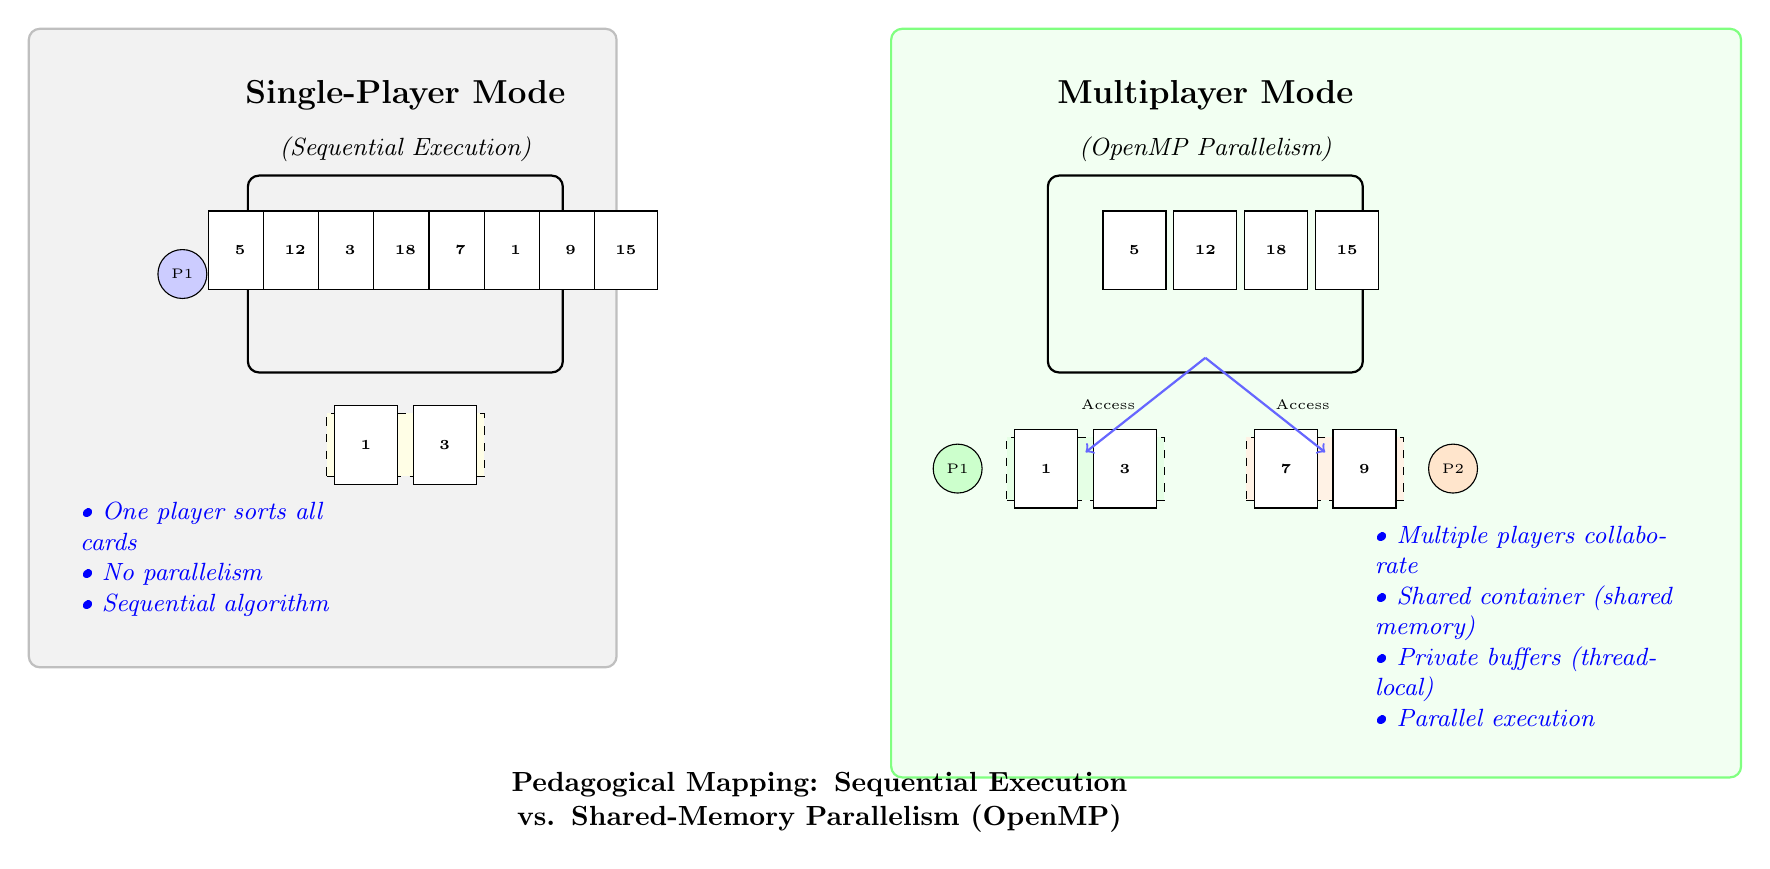
\begin{tikzpicture}[
    node distance=1cm,
    card/.style={rectangle, draw, fill=white, minimum width=0.8cm, minimum height=1cm, font=\tiny\bfseries},
    container/.style={rectangle, draw, thick, rounded corners, minimum width=4cm, minimum height=2.5cm},
    buffer/.style={rectangle, draw, dashed, fill=yellow!10, minimum width=2cm, minimum height=0.8cm},
    player/.style={circle, draw, fill=blue!20, minimum size=0.6cm, font=\tiny},
    label/.style={font=\bfseries\large},
    concept/.style={font=\small\itshape, text=blue}
]

% Sequential Mode (Left Side)
\node[label] (seq-title) {Single-Player Mode};
\node[font=\small\itshape, below=0.1cm of seq-title] {(Sequential Execution)};

\node[container, below=0.7cm of seq-title, label=below:\textbf{All Cards}] (seq-container) {};

% All cards in one container - properly positioned inside
\foreach \i/\num in {1/5, 2/12, 3/3, 4/18, 5/7, 6/1, 7/9, 8/15} {
    \node[card] at ([xshift=\i*0.7cm-2.8cm, yshift=0.3cm]seq-container.center) {\num};
}

% Single player working alone
\node[player, left=0.5cm of seq-container] (seq-player) {P1};

% Work buffer
\node[buffer, below=0.5cm of seq-container, label=below:Work Buffer] (seq-buffer) {};
\node[card] at ([xshift=-0.5cm]seq-buffer) {1};
\node[card] at ([xshift=0.5cm]seq-buffer) {3};

% Concepts - moved to the side
\node[concept, below left=0.2cm and -0.5cm of seq-buffer, text width=3.5cm, align=left] (seq-concepts) {
    • One player sorts all cards\\
    • No parallelism\\
    • Sequential algorithm
};

% OpenMP Mode (Right Side)
\node[label, right=6cm of seq-title] (openmp-title) {Multiplayer Mode};
\node[font=\small\itshape, below=0.1cm of openmp-title] {(OpenMP Parallelism)};

\node[container, below=0.7cm of openmp-title, label=below:\textbf{Shared Container}] (openmp-container) {};

% Cards in shared container - properly positioned inside
\foreach \i/\num in {1/5, 2/12, 3/18, 4/15} {
    \node[card] at ([xshift=\i*0.9cm-1.8cm, yshift=0.3cm]openmp-container.center) {\num};
}

% Player 1 buffer
\node[buffer, below left=0.8cm and -1.5cm of openmp-container, fill=green!10, label=below:Player 1 Private] (openmp-buffer1) {};
\node[card] at ([xshift=-0.5cm]openmp-buffer1) {1};
\node[card] at ([xshift=0.5cm]openmp-buffer1) {3};

% Player 2 buffer
\node[buffer, below right=0.8cm and -1.5cm of openmp-container, fill=orange!10, label=below:Player 2 Private] (openmp-buffer2) {};
\node[card] at ([xshift=-0.5cm]openmp-buffer2) {7};
\node[card] at ([xshift=0.5cm]openmp-buffer2) {9};

% Players
\node[player, left=0.3cm of openmp-buffer1, fill=green!20] (openmp-player1) {P1};
\node[player, right=0.3cm of openmp-buffer2, fill=orange!20] (openmp-player2) {P2};

% Bidirectional arrows showing shared access
\draw[->, thick, blue!60] ([yshift=0.2cm]openmp-container.south) --
    node[left, font=\tiny, text=black] {Access} ([yshift=-0.2cm]openmp-buffer1.north);
\draw[->, thick, blue!60] ([yshift=0.2cm]openmp-container.south) --
    node[right, font=\tiny, text=black] {Access} ([yshift=-0.2cm]openmp-buffer2.north);

% Concepts - moved to the side
\node[concept, below right=0.2cm and -0.5cm of openmp-buffer2, text width=4cm, align=left] (openmp-concepts) {
    • Multiple players collaborate\\
    • Shared container (shared memory)\\
    • Private buffers (thread-local)\\
    • Parallel execution
};

% Background boxes
\begin{scope}[on background layer]
    \node[fit=(seq-title)(seq-container)(seq-buffer)(seq-player)(seq-concepts),
          fill=gray!10, draw=gray!50, thick, rounded corners, inner sep=15pt] (seq-box) {};
    \node[fit=(openmp-title)(openmp-container)(openmp-buffer1)(openmp-buffer2)(openmp-player1)(openmp-player2)(openmp-concepts),
          fill=green!5, draw=green!50, thick, rounded corners, inner sep=15pt] (openmp-box) {};
\end{scope}

% Bottom comparison - centered between both background boxes
\path (seq-box.south) -- (openmp-box.south) coordinate[midway] (diagram-bottom-mid);
\node[below=0.5cm of diagram-bottom-mid, font=\bfseries, text width=13cm, align=center] {
    Pedagogical Mapping: Sequential Execution vs. Shared-Memory Parallelism (OpenMP)
};

\end{tikzpicture}
\end{document}
